\chapter{Detalles de Implementación}\label{chapter:implementation}
Este capítulo describe la implementación práctica del modelo teórico propuesto en el capítulo anterior. Se detallan las tecnologías utilizadas, las decisiones de diseño, y los desafíos enfrentados durante el desarrollo.

\section{Contexto Tecnol\'ogico}
Para la implementación de la propuesta, se utilizó el lenguaje \textit{JavaScript} tanto en la interfaz de usuario como en la API. Específicamente, para la API se empleó \textit{Supabase}, un servicio Baas (\textit{Backend} como servicio), que proporciona una base de datos \textit{PostgreSQL} y funciones \textit{serverless} ejecutadas en entornos \textit{JavaScript}. En cuanto a la creación de la interfaz de usuario, se utilizaron tecnologías web comunes como \textit{HTML}, \textit{CSS} y \textit{JavaScript}, todas integradas mediante el \textit{framework} \textit{Vue}. El uso de \textit{Vue} permitió agilizar el desarrollo de sitios web interactivos. 

\section{Arquitectura del Sistema}
El sistema utiliza una arquitectura cliente-servidor desacoplada. El \textit{frontend} (interfaz gr\'afica) cumple con el rol de ser la interfaz de usuario, la l\'ogica de presentaci\'on y gestionar la interacci\'on con el usuario. \textit{Supabase} \cite{supabase} act\'ua como \textit{backend}, cumple con el rol de procesamiento de datos, almacenamiento, autenticaci\'on y l\'ogica de negocio.

\subsection{Patrones y estilos arquitect\'onicos involucrados}
Enfoque \textit{serverless} (sin servidor), esto elimina la necesidad de gestionar un servidor tradicional y la necesidad de tener infraestructura propia. Este enfoque es prove\'ido a trav\'es del uso de \textit{Supabase} \cite{supabase}, esto aumenta la escalabilidad a la vez que reduce los tiempos de desarrollo.

\textit{Single Page Application} (SPA), aplicaci\'on de una sola p\'agina, es un enfoque en el que el navegador carga una sola p\'agina y actualiza el contenido din\'amicamente, esto mejora la reactividad de la web y hace m\'as din\'amica la interacci\'on con el usuario. Se obtiene este enfoque con la utilizaci\'on del \textit{framework} (marco de trabajo) de JavaScript \textit{Vue.js} \cite{vuejs} en el desarrollo de la interfaz gr\'afica, este  da las herramientas necesarias para desarrollar de manera pr\'actica y efectiva aplicaciones completas utilizando la arquitectura mencionada, se puede ver la interfaz gr\'afica en el Anexo No 11. (figuras de \ref{register-screen} a \ref{error-scans}).


\begin{table}[ht]
	\centering
	\caption{Características clave de la arquitectura Vue.js + \textit{Supabase} }
	\label{tab:arquitectura}
	\rowcolors{1}{}{gray!10} % Fondo alternado para filas
	\begin{tabular}{|p{2.1cm}|p{2cm}|p{5cm}|p{5cm}|} % Ajustar anchos según sea necesario
		\hline
		\rowcolor{gray!20} % Color del encabezado
		\textbf{Capa} & \textbf{Tecnología} & \textbf{Responsabilidad} & \textbf{Ejemplo} \\
		\hline
		
		Presentación & Vue.js & 
		Renderizar interfaz de usuario, manejar eventos del usuario, gestión de estado local & 
		Componentes Reactivos, formularios de registro, enrutamiento con Vue Router \\
		\hline
		
		Servicios & \textit{Supabase}  & 
		Proveer servicios backend vía API, gestión de autenticación, ejecutar operaciones CRUD & 
		Autenticación con OAuth, consultas a PostgreSQL, webhooks para notificaciones \\
		\hline
		
		Persistencia & PostgreSQL & 
		Almacenamiento transaccional, garantizar ACID, escalado vertical/horizontal & 
		Tabla de usuarios, registros de actividad, relaciones SQL complejas \\
		\hline
	\end{tabular}
\end{table}


\section{M\'odulos de la aplicaci\'on}

\subsection{Selección de la imagen}
\label{subsec:seleccion-imagen}

En ambas fases (registro y autenticación), el sistema presenta al usuario tres imágenes, ver figura \ref{fig:imagenes-sistema}, en orden aleatorio, de las cuales debe seleccionar aquella asociada a su contraseña. Este mecanismo añade una capa adicional de seguridad al evitar que los usuarios seleccionen siempre la misma imagen por dejadez o por la comodidad de tomar siempre la primera imagen de la lista, evitando as\'i que la selecci\'on de imagen sea predecible. 


\begin{figure}[ht]
	\centering
	\begin{minipage}[b]{0.3\textwidth}
		\centering
		
\includegraphics[width=\textwidth]{Graphics/disney.jpeg}
		\caption*{Imagen 1: Disney}
	\end{minipage}
	\hfill
	\begin{minipage}[b]{0.3\textwidth}
		\centering
		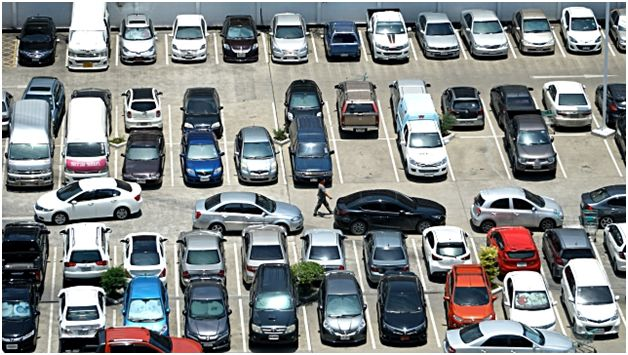
\includegraphics[width=\textwidth]{Graphics/cars.jpeg}
		\caption*{Imagen 3: Cars}
	\end{minipage}
	\hfill
		\begin{minipage}[b]{0.3\textwidth}
		\centering
		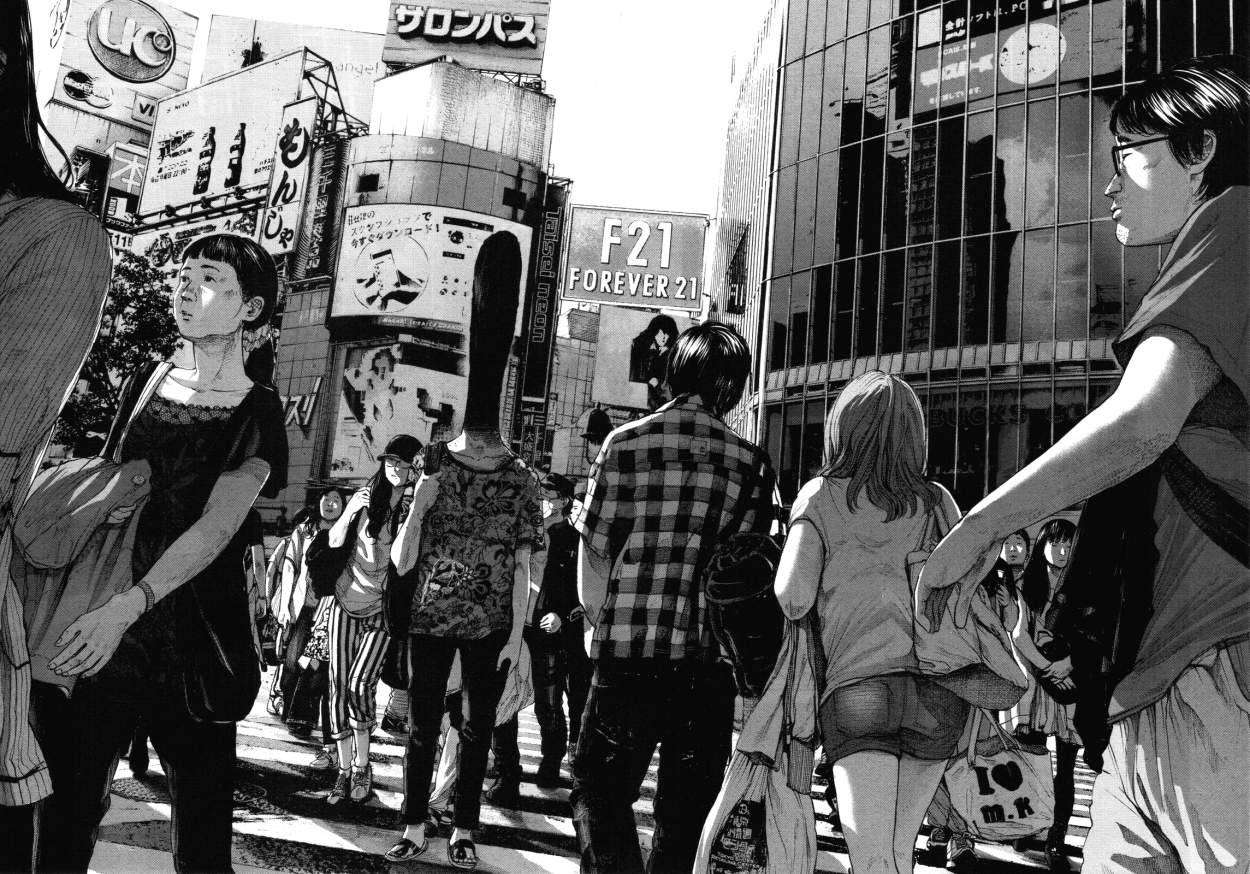
\includegraphics[width=\textwidth]{Graphics/japan.jpg}
		\caption*{Imagen 2: Japan}
	\end{minipage}
	
	\caption{Imágenes disponibles para la selección en el sistema}
	\label{fig:imagenes-sistema}
\end{figure}

La Tabla \ref{tab:uso-imagenes} muestra la distribución real del uso de imágenes según los datos de 33 usuarios. Se observa una preferencia por la imagen Disney (39.39\%), mientras que Japan y Cars presentan una distribución equitativa.


\begin{table}[ht]
	\centering
	\caption{Distribución de uso de imágenes en contraseñas (n = 33)}
	\label{tab:uso-imagenes}
	\begin{tabularx}{0.8\textwidth}{Xcc}
		\toprule
		\textbf{Imagen} & \textbf{Contraseñas} & \textbf{Frecuencia Relativa} \\
		\midrule
		Disney & 13 & 39.39\% \\
		Japan & 10 & 30.30\% \\
		Cars & 10 & 30.30\% \\
		\bottomrule
	\end{tabularx}
	\vspace{0.2cm}

\end{table}

\subsection{Captura de los puntos}
Para seleccionar los puntos se coloca la imagen seleccionada por el usuario de entre un conjunto prove\'ido por el sistema. De esta imagen se obtienen su tama\~no y posici\'on en la pantalla, de tal manera que al reaccionar al evento de \textit{click} del usuario se pueda calcular la regi\'on de la imagen que haya sido seleccionada, esto se puede entender de los ejemplos \ref{point-capture1} y \ref{point-capture2}. 


\begin{lstlisting}[style=mystyle, language=Java, breaklines=true, caption={C\'odigo de selecci\'on de coordenadas de pantalla}, label={point-capture1}, floatplacement=H]
  const { left, top, width, height } =
imagecontainer.value.getBoundingClientRect();
indicators.push({
	x: ((event.clientX - left) / width) * 100,
	y: ((event.clientY - top) / height) * 100,
});
\end{lstlisting}

\begin{lstlisting}[breaklines=true, language=Java, caption={C\'odigo de transformaci\'on en coordenadas de imagen}, label={point-capture2}, floatplacement=H]
	passwordInfo.points = e.map((point: Point) => {
		const { x, y } = point;
		return {
			x: Math.floor((x / 100) * passwordInfo.image.width),
			y: Math.floor((y / 100) * passwordInfo.image.height),
		};
		});
\end{lstlisting}

\subsection{Registro y autenticaci\'on}
\subsubsection{Proceso de Registro}
Durante la fase de registro, el usuario debe ingresar en dos ocasiones su contraseña gráfica (\textit{Passpoints}), ver Anexo No 11. (figuras \ref{register-screen},  \ref{screen-shapes-variety},\ref{error-scans}). Este mecanismo de doble verificación busca incrementar la memorabilidad de la secuencia de \textit{clicks}. Posteriormente, el sistema realiza una llamada a una \textit{edge function} de \textit{Supabase} , a la cual se transmiten:

\begin{itemize}
	\item Correo insertado por el usuario
	\item Nombre de usuario digitado
	\item Identificador de la imagen seleccionada
	\item Tolerancia utilizada 
	\item Ancho y alto de la imagen
	\item Coordenadas $(x,y)$ de los puntos seleccionados
\end{itemize}

Esta función se encarga de: 
\begin{enumerate}
	\item Discretizar la imagen, obteniendo los parámetros $\phi$  y $\varphi$ de cada punto.
	\item Generar el \textit{hash} de ambas instancias de la contraseña (original y de confirmación) utilizando el m\'etodo explicado en el cap\'itulo anterior.
	\item Validar la congruencia entre ambos \textit{hashes}.
	\item Utilizar los m\'odulos prove\'idos por \textit{Supabase}  para el registro y autenticaci\'on del usuario usando esta informaci\'on.
\end{enumerate}

Al proceso de \textit{hashing} se le agrega un n\'umero generado aleatoriamente criptogr\'aficamente seguro. Esto hace que los \textit{hashes} de contrase\~nas iguales sean diferentes y previene ataques de tipo \textit{Rainbow Tables}.

\subsubsection{Mecanismo de registro y autenticaci\'on}
El módulo de autenticación de \textit{Supabase}  emplea un esquema basado en \textit{JSON Web Tokens (JWT)} para:
\begin{itemize}
	\item Gestionar sesiones de usuario
	\item Verificar identidades en cada solicitud
	\item Mantener integridad en la comunicación cliente-servidor
\end{itemize}

Para integrar el sistema \textit{Passpoints} con este servicio:
\begin{itemize}
	\item Se utiliza el \textit{hash} generado del \textit{Passpoints} como contraseña textual en el registro y autenticaci\'on con \textit{Supabase} .
	\item Se preserva el requisito de entrada válida de \textit{Passpoints} para autenticaciones futuras.
	\item Se garantiza compatibilidad con el flujo estándar de OAuth 2.0, lo cual garantiza que se puedan seguir usando los servicios prove\'idos por \textit{Supabase} \cite{supabase}.
\end{itemize}


\begin{table}[ht]
	\centering
	\caption{Estructura de la tabla de usuarios}
	\label{tab:bd-esquema}
	\begin{tabularx}{\textwidth}{lX}
		\toprule
		\textbf{Tabla \texttt{user}} & \textbf{Descripción} \\
		\midrule
		\texttt{id} & Identificador único del usuario (UUID v4) \\
		\texttt{email} & Correo electrónico del usuario (único, formato validado) \\
		\texttt{password\_hash} & Hash de la contraseña gráfica \\
		\texttt{phi\_params} & Parámetros de cuantización espacial (JSON) \\
		\texttt{varphi\_params} & Parámetros de tolerancia (JSON) \\
		\texttt{salt} & Valor aleatorio criptográfico (256 bits) \\
		\texttt{tolerance\_radius} & Radio de tolerancia en píxeles (entero 8-32) \\
	
		\bottomrule
	\end{tabularx}
\end{table}


\begin{table}[ht]
	\centering
	\begin{tabularx}{\textwidth}{lX}
		\toprule
		\textbf{Tabla \texttt{Passwords}} & \textbf{Descripción} \\
		\midrule
		\texttt{user\_id} & Clave foránea a \texttt{user.id} \\
		\texttt{image\_id} & Identificador de la imagen base \\
		\texttt{tolerance} & Radio de tolerancia en píxeles \\
		\texttt{points} & Coordenadas $(x,y)$ en texto claro \\
		\texttt{discretization\_params} & $\phi$ y $\varphi$ en texto claro por cada punto (JSON) \\
		\bottomrule
	\end{tabularx}
\end{table}

\subsubsection{Nota de Seguridad}
La decisión de almacenar en texto claro:
\begin{itemize}
	\item Coordenadas de los puntos.
	\item Parámetros $\phi$ y $\varphi$.
	\item Informaci\'on de la imagen, identificador, ancho, alto.
\end{itemize}

Se restringe exclusivamente a fines académicos. En un entorno productivo se aplicarían las siguientes medidas:
\begin{itemize}
	\item Cifrado AES-256 de todos los parámetros sensibles.
	\item No se guardar\'ian las coordenadas originales de la contrase\~na.
	\item No se guardar\'ia la informaci\'on de la imagen utilizada.
\end{itemize}

\subsection{Flujo de Autenticación}
Durante la fase de autenticación, el usuario debe:

\begin{enumerate}
	\item Seleccionar la imagen utilizada durante el registro de entre tres opciones presentadas en orden aleatorio.
	\item Ingresar su contraseña gráfica (\textit{Passpoints
}) sobre la imagen seleccionada
\end{enumerate}

Este diseño incrementa la conciencia del usuario sobre su elección y reduce la predictibilidad del sistema ante posibles ataques.

\subsubsection{Mecanismos de Seguridad}
El sistema implementa las siguientes protecciones:

\begin{itemize}
	\item Ocultamiento de regiones de tolerancia: Los indicadores visuales (recuadros rojos del tama\~no de la regi\'on de tolerancia) se deshabilitan por defecto para prevenir ataques \textit{shoulder surfing}, aunque el usuario puede habilitarlos.
	\item \textit{Edge function} especializada: Valida las credenciales mediante el flujo:
	\begin{enumerate}
		\item Verificación de existencia del usuario en la base de datos.
		\item Recuperación de parámetros almacenados ($\varphi$, valor aleatorio $salt$, tolerancia $tolerance$, y \textit{hash} original), valores de la tabla \ref{tab:bd-esquema}
		\item Recomputación del \textit{hash} usando el método de discretización descrito en el Capítulo anterior.
		\item Verificaci\'on de la autenticidad de la contrase\~na usando el m\'odulo de autenticaci\'on de \textit{Supabase}.
	\end{enumerate}
\end{itemize}

\begin{table}[ht]
	\centering
	\caption{Parámetros de verificación en autenticación}
	\label{tab:parametros-verificacion}
	\begin{tabularx}{\textwidth}{lXl}
		\toprule
		\textbf{Parámetro} & \textbf{Descripción} & \textbf{Tipo} \\
		\midrule
		$\varphi$ & Lista de $\phi$, $\varphi$ de los puntos & JSON \\
		$c$ & Valor aleatorio  (\textit{salt}) & CHAR (256) \\
		$t$ & Radio de tolerancia & Entero 32 bits \\
		$h$ & \textit{Hash} & \texttt{CHAR(60)} \\
		\bottomrule
	\end{tabularx}
\end{table}

\subsubsection{Gestión de Sesiones}
El servicio de autenticación de \textit{Supabase}  emplea \textit{JSON Web Tokens (JWT)} para:

\begin{itemize}
	\item Generar credenciales temporales con expiración.
	\item Gestionar la validez de los \textit{tokens} en cada petici\'on y restringir acceso a los servicios en funci\'on de las pol\'iticas de seguridad definidas.
	\item Almacenar el estado de sesión en \textit{cookies} HttpOnly/Secure de lado del usuario, a trav\'es de uso de su cliente de JavaScript en la interfaz.
\end{itemize}

La validación resulta en:
\begin{itemize}
	\item Creación de sesión con \textit{token} de acceso/refresh en caso de ser exitosa.
	\item Entrada de un registro en la tabla \textit{auth-passwords} donde se guardan los puntos usados en el intento de autenticaci\'on y el resultado del mismo.
	\item Entrega al cliente de credenciales y datos de sesi\'on para acceder a su informaci\'on en el sistema.
\end{itemize}

